\documentclass[a4paper,fontset = windows]{ctexbook}
\usepackage[user=teacher]{cexam}
\usepackage[margin=2cm]{geometry}
\usepackage{xifthen}
\usepackage{calc}
\usepackage{graphicx}
\usepackage{tikz}
\usetikzlibrary{patterns}
\usepackage{amsthm}
\usepackage{amsfonts}
\usepackage{amssymb}
\usepackage{mathtools}
\usepackage{amsmath}
\begin{document}
\chapter{基本排版程序}


%\ExplSyntaxOn
%\parindent=0pt
\begin{proof}
   考虑下凸函数$e^x$,$x\in R$,由琴生不等式可得
   \[
      e^{\alpha_1x_1+\alpha_2x_2+\cdots +\alpha_nx_n}
      \leqslant
      \alpha_1e^{x_1}+\alpha_2e^{x_2}+\cdots +\alpha_ne^{x_n}
   \]
   在上式中取$a_i=e^{x_i}$,则$a_i>0$ ,于是上式化为
   \[
      a_1^{\alpha_1}a_2^{\alpha_2}\cdots a_n^{\alpha_n}
      \leqslant
      \alpha_1 a_1+\alpha_2 a_2+\cdots +\alpha_n a_n
   \]
   如果$\alpha_1>1$,$\alpha_i<0$,$(i=2,3,\dots,n)$,同时也满足$\sum \alpha_i=1$则按Jensen不等式可知,不等号改变方向,即
   \[
      a_1^{\alpha_1}a_2^{\alpha_2}\cdots a_n^{\alpha_n}
      \geqslant
      \alpha_1 a_1+\alpha_2 a_2+\cdots +\alpha_n a_n
   \]

\end{proof}


\begin{tiankong}
   1.一质量为$m$的小球,用长为$l$的轻绳悬挂于$O$点.小球在水平拉力$F$的作用下,从平衡位置$P$点很缓慢地移动到$Q$点,如
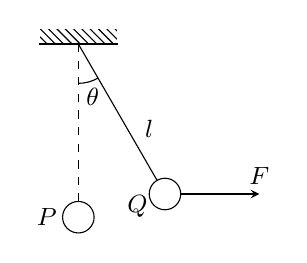
\begin{tikzpicture}
  \draw [color=white,pattern=north west lines] (-0.5,0) rectangle (0.5,0.2);
  \draw (-0.5,0)--(0.5,0); 
  \draw[dashed] (0,0)--(0,-2);
  \draw (0,-2.2) circle [radius=0.2];
  \draw (0,0)--(300:2);
  \draw (300:2.2) circle [radius=0.2];
  \draw[->,>=stealth] (300:2.2)++(0.2,0)--++(1,0) node [anchor=south]{\small $F$};
  \draw (270:0.5) arc (270:300:0.5);
  \draw (285:0.7) node {\small $\theta$};
  \draw (-0.4,-2.2) node {\small $P$};
  \draw (290:2.2) node {\small $Q$};
  \draw (310:1.4) node {\small $l$};
\end{tikzpicture}
所示,则拉力F所做的功为多少?
所示,则拉力F所做的功为多少?
所示,则拉力F所做的功为多少?
所示,则拉力F所做的功为多少?
所示,则拉力F所做的功为多少?
所示,则拉力F所做的功为多少?
所示,则拉力F所做的功为多少?
所示,则拉力F所做的功为多少?
所示,则拉力F所做的功为多少?
所示,则拉力F所做的功为多少?
所示,则拉力F所做的功为多少?
所示,则拉力F所做的功为多少?
所示,则拉力F所做的功为多少?
所示,则拉力F所做的功为多少?

\end{tiankong}
%\makeanswer

\end{document}
